% ОБЯЗАТЕЛЬНО ИМЕННО ТАКОЙ documentclass!
% (Основной кегль = 14pt, поэтому необходим extsizes)
% Формат, разумеется, А4
% article потому что стандарт не подразумевает разделов
% Глава = section, Параграф = subsection
% (понятия "глава" и "параграф" из стандарта)
\documentclass[a4paper,article,14pt]{extarticle}

% Подключаем главный пакет со всем необходимым
\usepackage{spbudiploma_tempora}

% Пакеты по желанию (самые распространенные)
% Хитрые мат. символы
\usepackage{euscript}
% Таблицы
\usepackage{longtable}
\usepackage{makecell}
% Картинки (можно встявлять даже pdf)
\usepackage[pdftex]{graphicx}

\usepackage{amsthm,amssymb, amsmath}
\usepackage{textcomp}


\begin{document}

% Титульник в файле titlepage.tex
% Титульный лист диплома СПбГУ
% Временное удаление foot на titlepage
\newgeometry{left=30mm, top=20mm, right=15mm, bottom=20mm, nohead, nofoot}
\begin{titlepage}
\begin{center}
% Первый символ съедается, первым знаком поставлен Ы
\textbf{Санкт--Петербургский}
\textbf{государственный университет}

\vspace{35mm}

\textbf{\textit{\large Тихонков Сергей Алексеевич}} \\[8mm]
% Название
\textbf{\large Выпускная квалификационная работа}\\[3mm]
\textbf{\textit{\large Исследование и применение алгоритмов на базе консенсуса для распределенного обучения нейронных сетей}}

\vspace{20mm}
% Булшит
Уровень образования: бакалавриат\\
Направление 02.03.02 «Фундаментальная информатика и информационные технологии»\\
Основная образовательная программа СВ.5003.2017
«Программирование и информационные технологии»\\
Профиль «Автоматизация научных исследований»\\[30mm]


% Научный руководитель, рецензент
% Сходить в уч отдел и узнать, правильно ли
\begin{flushright}
{Научный руководитель:} \\
профессор, кафедра математического моделирования энергетических систем, д.ф. - м.н.  Крылатов~Александр Юрьевич
\end{flushright}
\begin{flushright}
{Рецензент:} \\
доцент, зав. каф. компьютерных технологий и систем, к.ф. - м.н.  Погожев~Сергей Владимирович
\end{flushright}

\vfill 

{Санкт-Петербург}
\par{\the\year{} г.}
\end{center}
\end{titlepage}
% Возвращаем настройки geometry обратно (то, что объявлено в преамбуле)
\restoregeometry
% Добавляем 1 к счетчику страниц ПОСЛЕ titlepage, чтобы исключить 
% влияние titlepage environment
\addtocounter{page}{1}


% Содержание
\tableofcontents
\pagebreak

\specialsection{Введение}
С каждым годом растет количество
накопленных человечеством данных. Современное аппаратное обеспечение часто не позволяет проводить вычисления
с большим количеством данных на одной машине. Это часто связано во-первых, с ограниченным объемом оперативной памяти компьютера,
а во-вторых, с ограниченным временным на решение конкретной задачи. Область машинного обучения испытывает обе перечисленные проблемы.
Часто для достижения требуемого результата необходимо обучение нейронной сети с множеством параметров на огромном объеме данных.
Это препятствует прогрессу в исследованиях и разработках.  В связи с этим существует потребность в методах распределенного обучения.
Они позволяют не ограничиваться мощностями одной машины при конструировании новых методов в машинном обучении
и ускоряют уже существующие решения.

Помимо этого на практике часто возникает потребность обрабатывать информацию разной степени приватности. В некоторых случаях
при обучении нейронной сети используются данные, распространение которых запрещено или нежелательно. Отличным примером этого
является какой-либо совместный проект двух банков, в ходе которого они хотят решить общую задачу, но не могут передать, пусть даже
и обезличенные, данные своих клиентов друг другу. В этом случае возникает необходимость использовать методы распределенного обучения, которые
обеспечивают изоляцию данных.

Топология сети и методы взаимодействия узлов являются важными свойствами распределенных систем. Не всегда вычислительные
кластеры имеют регулярную структуру, часто доступные вычислительные ресурсы представляют собой гетерогенную компьютерную сеть,
где пропускная способность каналов связи и мощности каждого узла могут сильно отличаться. В этом случае применяемые методы распределенного
обучения должны быть устойчивы к неоднородности сети.

В данной работе проводится краткий обзор основных методов распределенного обучения нейронных сетей и исследование
возможности применения алгоритма среднего консенсуса для распределенного обучения с изоляцией данных. Также рассматривается
способность исследуемого алгоритма корректно решать задачу в сети с неоднородной вычислительной мощностью узлов.

\specialsection{Постановка задачи}

\section{Обзор}
\subsection{Обзор раз}
Ненумерованная формула:

\begin{equation}
    \begin{pmatrix} \dot{\varphi}\\ \dot{\theta} \\ \dot{\psi} \end{pmatrix}
    = \begin{pmatrix}
        cos(\theta)cos(\psi) & -sin(\psi) & 0 \\
        cos(\theta)sin(\psi) & cos(\psi)  & 0 \\
        -sin(\theta)         & 0         &  1
    \end{pmatrix}^{-1}
    \begin{pmatrix} \omega_x\\ \omega_y \\ \omega_z \end{pmatrix}.
\end{equation}

Нумерованная формула:

\begin{equation} \label{eq:my_ref}
    i^2 = -1.
\end{equation}

Тест ссылки на формулу~\ref{eq:my_ref}!

\subsection{Обзор два}

\subsection{Обзор три}
Ниже тестируется очень большая таблица на несколько страниц

\begin{center}
    \begin{longtable}{|p{2cm}|p{3cm}|p{7cm}|p{3cm}|}
    \caption{Заголовок таблицы}\\
    \hline
    1 & 2 & 3 & 4\\
    \hline
    2 & 2 & 3 & 4\\
    \hline
    3 & 2 & 3 & 4\\
    \hline
    4 & 2 & 3 & 4\\
    \hline
    5 & 2 & 3 & 4\\
    \hline
    6 & 2 & 3 & 4\\
    \hline
    7 & 2 & 3 & 4\\
    \hline
    8 & 2 & 3 & 4\\
    \hline
    9 & 2 & 3 & 4\\
    \hline
    10 & 2 & 3 & 4\\
    \hline


    \end{longtable}
\end{center}


А также тестируется счетчик таблиц, жирные и двойные линии.

\begin{center}
    \begin{longtable}{|p{2cm}||p{3cm}|p{7cm}|p{3cm}|}
    \caption{Заголовок таблицы нумер 2}\\
    \hline
    1 & 2 & 3 & 4\\
    \hline
    2 & 2 & 3 & 4\\
    \hline
    3 & 2 & очень жирная ячейка \par с переносом (работаеттт!) & 4\\
    \hline
    4 & 2 & 3 & 4\\
    \hline
    5 & 2 & 3 & 4\\
    \hline
    6 & 2 & 3 & 4\\
    \hline
    7 & 2 & 3 & 4\\
    \hline
    8 & 2 & 3 & 4\\
    \hline
    9 & 2 & 3 & 4\\
    \hline
    10 & 2 & 3 & 4\\
    \hline


    \end{longtable}
\end{center}

\section{Консенсус}
\subsection{Теория}
\subsection{Fast averaging}

\pagebreak
\section{Алгоритм}
\subsection{Средний консенсус}
\subsection{Взвешенный консенсус}

\section{Эксперименты}
\subsection{Выбор модели и датасета}
\subsection{Преобразование данных}
\subsection{LSR}
\subsection{warmup}
\subsection{Топология сети}
Про экспандеры, разное количество диагоналей в цикле и вцелом про то какие топологии хорошие

\subsection{Анализ экспериментов}
\begin{figure}[ht]
\begin{center}
\scalebox{0.4}{
   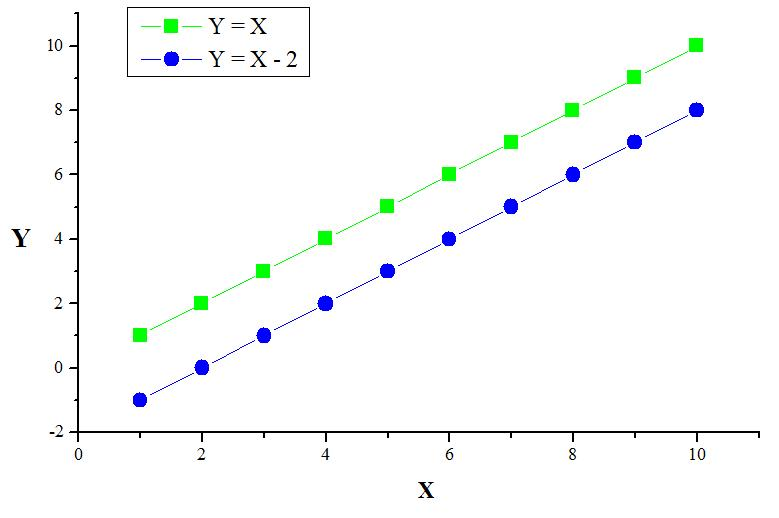
\includegraphics{examples/images/graph.jpg}
}

\caption{
\label{graph-fig}
     Линейные функции.}
\end {center}
\end {figure}
Ссылаемся на график ~\ref{graph-fig}.
Ссылка на статью: \cite{voc}, \cite{vo2}

\specialsection{Выводы}
Жизнь --- тлен.
\pagebreak

\specialsection{Заключение}

% Библиография в cpsconf стиле
% Аргумент {1} ниже включает переопределенный стиль с выравниванием слева
\begin{thebibliography}{1}
\bibitem{voc} Griffin D.W., Lim J.S. \flqq Multiband excitation vocoder\frqq. IEEE ASSP-36 (8), 1988, pp. 1223-1235.
\bibitem{vo2} Griffin D.W., Lim J.S. \flqq Multiband excitation vocoder\frqq. IEEE ASSP-36 (8), 1988, pp. 1223-1235.
\end{thebibliography}
\end{document}